\begin{frame}
\begin{columns}[c]
\begin{column}{0.5\textwidth}
\begin{block}{\textbf{Observe gene expression}}
\begin{itemize}
\item from transcript counts as in RNA-seq to qualitative organismal phenotypic characteristics such as coat color in mice or wing shape in flies
\item regardless of the level of observation the total number of \textbf{phenotype values} under consideration can be indexed as $P = \{ 1, \ldots, p \} $
\end{itemize}
\end{block}
\end{column}
\begin{column}{0.5\textwidth}
\begin{center}
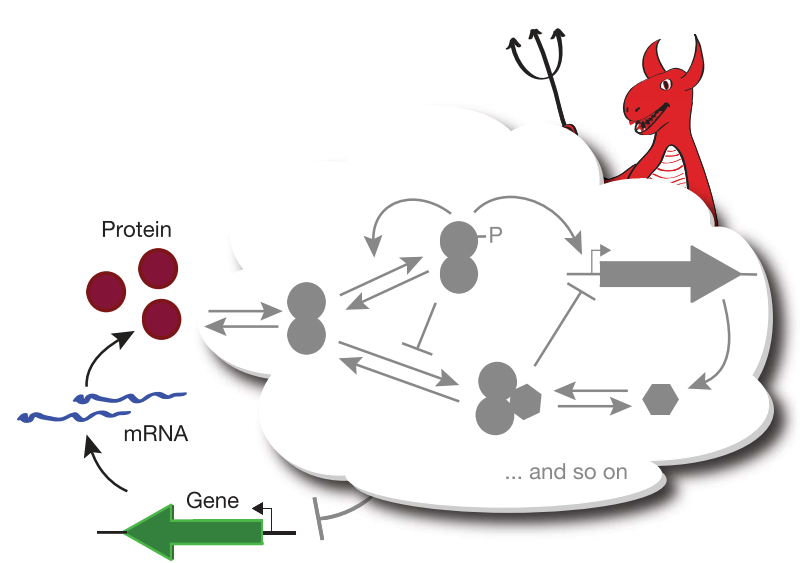
\includegraphics[width=1.0\textwidth]{fig/geneexpressiondemon.png}
\end{center}
\end{column}
\end{columns}
\end{frame}
